%standard 8.2
%week 7


%start_of_questions


%new_question
%%%%%%%%%%%%%%%%%%%%%
	% Problem 1
	% Difficulty: 2
%%%%%%%%%%%%%%%%%%%%%
	\item 	
		%https://edabit.com/challenge/vTGXrd5ntYRk3t6Ma
		An isogram is a word that has no duplicate letters. Write a \textbf{function} that takes a string $word$ 
		and returns either True or False depending on whether or not it's an isogram.

		\textbf{Examples:}		
		\begin{itemize}
			\item  is\_isogram(\csq{algorism}) $\rightarrow$ True
			\item  is\_isogram(\csq{password}) $\rightarrow$ False
			\item  is\_isogram(\csq{consecutive}) $\rightarrow$ False
		\end{itemize}


%new_question
%%%%%%%%%%%%%%%%%%%%%
	% Problem 2
	% Difficulty: 2
%%%%%%%%%%%%%%%%%%%%%
	\item 	
		In each input list, every number repeats at least once, except for one. Write a \textbf{function} that takes an array $numbers$
		 and returns the single unique number.

		\textbf{Examples:}		
		\begin{itemize}
			\item  find\_unique([1, 2, 2, 3, 3, 4, 4]) $\rightarrow$ 1,
			\item  find\_unique([7, 8, 8, 9, 9, 10, 10]) $\rightarrow$ 7,
			\item  find\_unique([5, 6, 6, 7, 7, 8, 8, 5, 9]) $\rightarrow$ 9
		\end{itemize}



%new_question
%%%%%%%%%%%%%%%%%%%%%
	% Problem 3
	% Difficulty: 2
%%%%%%%%%%%%%%%%%%%%%
	\item 	
		%https://edabit.com/challenge/yL5WmWTCNwwb4GnR7
		In each input list, every number repeats at least once, except for two. Write a \textbf{function} that takes an array $numbers$
		 and returns the two unique numbers.

		\textbf{Examples:}		
		\begin{itemize}
			\item  return\_unique([1, 9, 8, 8, 7, 6, 1, 6]) $\rightarrow$ [9, 7],
			\item  return\_unique([5, 5, 2, 4, 4, 4, 9, 9, 9, 1]) $\rightarrow$ [2, 1],
			\item  return\_unique([9, 5, 6, 8, 7, 7, 1, 1, 1, 1, 1, 9, 8]) $\rightarrow$ [5, 6]
		\end{itemize}




%new_question
%%%%%%%%%%%%%%%%%%%%%
	% Problem 9
	% Difficulty: 2
%%%%%%%%%%%%%%%%%%%%%
	%paper-based
	\item 	
		Below is a receipt from my recent lunch order.
		\begin{enumerate}
			\item Initialize an empty dictionary named receipt, and then add the contents of 
				the receipt as key-value pairs.
			\item Using the dictionary you created in part a, write code that prints the 
				total cost of all the items on the receipt.  The code should work regardless
				of the contents of the receipt. (meaning don't write print(6+12+3))
		\end{enumerate}	
		\begin{center}
		        \begin{tabular}{l|c}
		            \textbf{Item} & \textbf{Price} \\ \hline
		            Side Salad & \$6 \\
		            Chicken Parm & \$12 \\
		            Cookie & \$3 \\
		        \end{tabular}
		\end{center}

%new_question
%%%%%%%%%%%%%%%%%%%%%
	% Problem 10
	% Difficulty: 2
%%%%%%%%%%%%%%%%%%%%%
	%paper-based
	\item 	
		Below is the menu from my favorite restaurant.
		\begin{enumerate}
			\item Initialize an empty dictionary named menu, and then add the contents of 
				the menu as key-value pairs.
			\item Using the dictionary you created in part a, write code that prints 
			each of the items on the menu as key-value pairs.  The code should work 
			regardless of the contents of the receipt. 
			(meaning don't write print(\csq{burger}, 10))
		\end{enumerate}		
		\begin{center}
		    \begin{minipage}{.3\textwidth}
		        \begin{tabular}{l|c}
		            \textbf{Item} & \textbf{Price} \\ \hline
		            burger & \$10 \\
		            fries & \$4 \\
		            soda & \$3 \\
		        \end{tabular}
		    \end{minipage}
		    \begin{minipage}{.5\textwidth}
				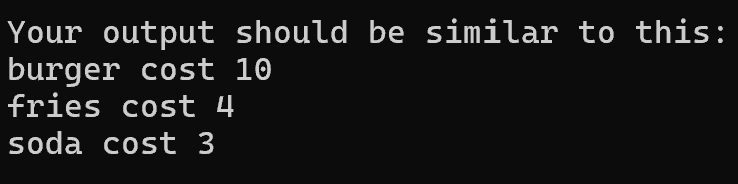
\includegraphics[scale=0.8]{./imgs/menu_output.png}
		    \end{minipage}
		\end{center}





%new_question
%%%%%%%%%%%%%%%%%%%%%
	% Problem 13
	% Difficulty: 2
%%%%%%%%%%%%%%%%%%%%%
\item
	Write a \textbf{function} that takes a dictionary, called $sales$, where the keys are product names and the values are the number of units sold. 
	The function should return the total number of products sold.

	\textbf{Examples:}  
	\begin{itemize}  
		\item total\_sales(\{\csq{Laptop}: 5, \csq{Phone}: 10, \csq{Tablet}: 3\}) $\rightarrow$ 18
		\item total\_sales(\{\csq{Shoes}: 20, \csq{Hats}: 15, \csq{Jackets}: 10\}) $\rightarrow$ 45
		\item total\_sales(\{\csq{Book}: 1, \csq{Pen}: 2, \csq{Notebook}: 1\}) $\rightarrow$ 4
	\end{itemize}



%new_question
%%%%%%%%%%%%%%%%%%%%%
	% Problem 15
	% Difficulty: 2
%%%%%%%%%%%%%%%%%%%%%
\item
	Write a \textbf{function} that takes a dictionary, called $donations$, where the keys are donor names and the values are the amount donated. 
	The function should return the total amount donated.
	
	\textbf{Examples:}  
	\begin{itemize}  
		\item total\_donations(\{\csq{John}: 100, \csq{Sarah}: 200, \csq{Mike}: 50\}) $\rightarrow$ 350
		\item total\_donations(\{\csq{Anna}: 500, \csq{Tom}: 1000, \csq{Jerry}: 1500\}) $\rightarrow$ 3000
		\item total\_donations(\{\csq{Chris}: 25, \csq{Alex}: 30, \csq{Morgan}: 45\}) $\rightarrow$ 100
	\end{itemize}




%new_question
%%%%%%%%%%%%%%%%%%%%%
	% Problem 16
	% Difficulty: 2
%%%%%%%%%%%%%%%%%%%%%
\item
	Write a \textbf{function} that takes a list of \textbf{fruits} and returns the total \textbf{caloric value} of the fruits consumed. You may use the following 
	dictionary named $calories$:
	\begin{center}
		\textit{calories} = \{ \csq{apple} : 95, \csq{banana} : 105, \csq{orange} : 62, 
			\csq{grape} 3, \csq{pear} : 102\}
	\end{center}
	Hint: You can calculate the total calories by summing up the caloric values of all valid 
	fruits in the list. You may assume the \textit{calories} dictionary is defined in your code.  
	You don't need to rewrite it.
	
	
	\textbf{Examples:}  
	\begin{itemize}  
		\item total\_calories([\csq{apple}, \csq{banana}, \csq{orange}]) 
			$\rightarrow$ 262 (since 95 + 105 + 62 = 262)
		\item total\_calories([\csq{grape}, \csq{grape}, \csq{grape}, \csq{grape}, \csq{grape}]) 
			$\rightarrow$ 15
		\item total\_calories([\csq{banana}, \csq{pear}, \csq{apple}]) $\rightarrow$ 302
	\end{itemize}


%new_question
%%%%%%%%%%%%%%%%%%%%%
	% Problem 17
	% Difficulty: 2
%%%%%%%%%%%%%%%%%%%%%
\item
	Write a \textbf{function} that takes a list of \textbf{ingredients} and returns the total 
	\textbf{cost} of making a recipe. You may use the following dictionary named $prices$:
	\begin{center}
		prices = \{ \csq{flour} : 2.50, \csq{sugar} : 1.80, \csq{eggs} : 3.00, \csq{milk} : 2.00, 
			\csq{butter} : 2.75, \csq{vanilla} : 4.50, \csq{chocolate} : 5.00 \}
	\end{center}
	Hint: You can calculate the total cost by summing up the prices of all valid ingredients in 
	the list.  You may assume the \textit{prices} dictionary is defined in your code.  You don't 
	need to rewrite it.
	
	\textbf{Examples:}  
	\begin{itemize}  
		\item total\_cost([\csq{flour}, \csq{sugar}, \csq{eggs}, \csq{butter}]) $\rightarrow$ 10.05
		\item total\_cost([\csq{milk}, \csq{vanilla}, \csq{chocolate}]) $\rightarrow$ 11.50
		\item total\_cost([\csq{eggs}, \csq{eggs}, \csq{flour}, \csq{sugar}]) $\rightarrow$ 10.30
	\end{itemize}



%new_question
%%%%%%%%%%%%%%%%%%%%%
	% Problem 18
	% Difficulty: 2
%%%%%%%%%%%%%%%%%%%%%
%https://leetcode.com/problems/majority-element/description/?envType=problem-list-v2&envId=hash-table
\item
	Write a \textbf{function} named \textit{majority\_elment} that takes a list of integers named \textit{nums} and returns the majority element. The majority element is the element that has at least half of the occurrences. You may assume that the majority element always exists and is unique.
	
	\textbf{Examples:}  
	\begin{itemize}  
		\item majority\_elment([3,2,3]) $\rightarrow$ 3
		\item majority\_elment([2,2,1,1,1,2,2]) $\rightarrow$ 2
		\item majority\_elment([2,2,3,2,1,2,1,4,4,1,2,2]) $\rightarrow$ 2
	\end{itemize}

%end_of_questions
%make sure to leave at least one blank line below

